\chapter{Raisonnement par Récurrence et Suites}

Ce premier chapitre pose les bases de l'analyse en Terminale. Nous allons étudier un nouveau type de raisonnement, le raisonnement par récurrence, puis nous l'appliquerons à l'étude des limites de suites et de leur convergence.

\section{Le Raisonnement par Récurrence}

Le raisonnement par récurrence permet de démontrer qu'une propriété $P(n)$, dépendant d'un entier naturel $n$, est vraie pour tout entier $n \ge n_0$.

\begin{definition}[Principe de récurrence]
Soit $n_0 \in \N$ et $P(n)$ une propriété définie pour tout entier $n \ge n_0$.
Si les deux conditions suivantes sont satisfaites :
\begin{enumerate}
    \item \textbf{Initialisation} : La propriété est vraie au rang initial $n_0$, c'est-à-dire que $P(n_0)$ est vraie.
    \item \textbf{Hérédité} : Pour tout entier $k \ge n_0$, si la propriété est vraie à un rang $k$ (hypothèse de récurrence), alors elle est vraie au rang suivant $k+1$.
\end{enumerate}
Alors, la propriété $P(n)$ est vraie pour tout entier $n \ge n_0$.
\end{definition}

\begin{methode}[Rédiger une récurrence]
Pour rédiger une démonstration par récurrence, on suit rigoureusement trois étapes :
\begin{itemize}
    \item \textbf{Initialisation} : On montre que la propriété est vraie pour le premier rang $n = n_0$.
    \item \textbf{Hérédité} : On pose l'hypothèse de récurrence : « Supposons que pour un entier $k \ge n_0$, la propriété $P(k)$ soit vraie. » On cherche ensuite à prouver sous cette hypothèse que la propriété $P(k+1)$ est vraie.
    \item \textbf{Conclusion} : On conclut : « La propriété est initialisée et héréditaire, donc par récurrence, $P(n)$ est vraie pour tout $n \ge n_0$. »
\end{itemize}
\end{methode}

\begin{exemple}[Somme des premiers entiers]
Montrons par récurrence que pour tout $n \ge 1$ :
\[
S_n = \sum_{i=1}^n i = 1 + 2 + \dots + n = \frac{n(n+1)}{2}
\]
\textbf{Initialisation} : Pour $n = 1$, $S_1 = 1$ et $\frac{1(1+1)}{2} = 1$. L'initialisation est vérifiée.

\textbf{Hérédité} : Supposons la propriété vraie pour un entier $k \ge 1$ : $S_k = \frac{k(k+1)}{2}$.
Montrons qu'elle est vraie pour $k+1$ :
\[
S_{k+1} = S_k + (k+1) = \frac{k(k+1)}{2} + (k+1) = (k+1)\left( \frac{k}{2} + 1 \right) = \frac{(k+1)(k+2)}{2}
\]
L'hérédité est prouvée.

\textbf{Conclusion} : Pour tout $n \ge 1$, $\sum_{i=1}^n i = \frac{n(n+1)}{2}$.
\end{exemple}

\section{Limites de Suites}

\subsection{Limite infinie}

\begin{definition}[Limite $+\infty$ et $-\infty$]
\begin{itemize}
    \item On dit qu'une suite $(u_n)$ a pour limite $+\infty$ si tout intervalle de la forme $]A, +\infty[$ (où $A \in \R$) contient tous les termes de la suite à partir d'un certain rang. On note alors :
    \[
    \lim_{n \to +\infty} u_n = +\infty
    \]
    \item De même, on dit qu'une suite $(u_n)$ a pour limite $-\infty$ si tout intervalle de la forme $]-\infty, B[$ (où $B \in \R$) contient tous les termes de la suite à partir d'un certain rang.
\end{itemize}
\end{definition}

\subsection{Limite finie et convergence}

\begin{definition}[Suite convergente]
On dit qu'une suite $(u_n)$ a pour limite le réel $L$ si tout intervalle ouvert contenant $L$ contient tous les termes de la suite à partir d'un certain rang. On dit alors que la suite $(u_n)$ est \textbf{convergente} vers $L$ et on note :
\[
\lim_{n \to +\infty} u_n = L
\]
Une suite qui ne converge pas vers une limite finie est dite \textbf{divergente}.
\end{definition}

\begin{propriete}[Limites des suites géométriques]
Soit $q$ un nombre réel et la suite géométrique $u_n = q^n$.
\begin{itemize}
    \item Si $q > 1$, alors $\lim_{n \to +\infty} q^n = +\infty$.
    \item Si $-1 < q < 1$, alors la suite $(q^n)$ converge vers $0$.
    \item Si $q = 1$, la suite est constante et converge vers $1$.
    \item Si $q \le -1$, la suite $(q^n)$ n'admet pas de limite.
\end{itemize}
\end{propriete}

\section{Théorèmes de Convergence}

\subsection{Théorèmes de comparaison}

\begin{theoreme}[Théorème des Gendarmes]
Soit $(u_n)$, $(v_n)$ et $(w_n)$ trois suites. Supposons qu'à partir d'un certain rang :
\[
u_n \le v_n \le w_n
\]
Si $\lim_{n \to +\infty} u_n = \lim_{n \to +\infty} w_n = L$ (avec $L \in \R$), alors la suite $(v_n)$ converge et sa limite est $L$.
\end{theoreme}

\begin{theoreme}[Théorèmes de comparaison pour l'infini]
Soit $(u_n)$ et $(v_n)$ deux suites. Supposons qu'à partir d'un certain rang $u_n \le v_n$.
\begin{itemize}
    \item Si $\lim_{n \to +\infty} u_n = +\infty$, alors $\lim_{n \to +\infty} v_n = +\infty$.
    \item Si $\lim_{n \to +\infty} v_n = -\infty$, alors $\lim_{n \to +\infty} u_n = -\infty$.
\end{itemize}
\end{theoreme}

\subsection{Convergence des suites monotones}

\begin{definition}[Suite majorée, minorée, bornée]
\begin{itemize}
    \item Une suite $(u_n)$ est \textbf{majorée} s'il existe un réel $M$ tel que pour tout $n \in \N$, $u_n \le M$.
    \item Une suite $(u_n)$ est \textbf{minorée} s'il existe un réel $m$ tel que pour tout $n \in \N$, $u_n \ge m$.
    \item Une suite est \textbf{bornée} si elle est à la fois majorée et minorée.
\end{itemize}
\end{definition}

\begin{theoreme}[Théorème de convergence monotone]
\begin{itemize}
    \item Toute suite croissante et majorée est convergente.
    \item Toute suite décroissante et minorée est convergente.
\end{itemize}
\end{theoreme}

\begin{exemple}[Suite définie par $u_{n+1} = f(u_n)$]
Soit la suite définie par $u_0 = 0$ et pour tout $n \in \N$, $u_{n+1} = \sqrt{u_n + 2}$.
La fonction associée est $f(x) = \sqrt{x+2}$. On peut étudier graphiquement la convergence de cette suite grâce à la méthode de la toile d'araignée (cobweb plot).

\begin{center}
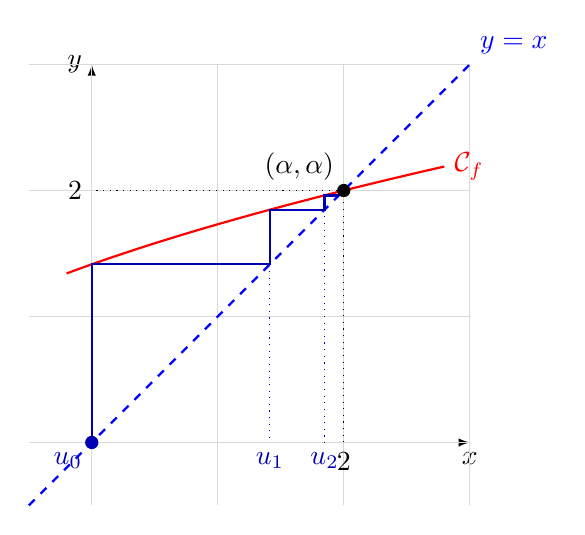
\begin{tikzpicture}[scale=1.6]
  \draw[->,>=latex] (-0.5,0) -- (3,0) node[below] {$x$};
  \draw[->,>=latex] (0,-0.5) -- (0,3) node[left] {$y$};
  \draw[gray!30,very thin] (-0.5,-0.5) grid (3,3);
  
  \draw[dashed, blue, thick] (-0.5,-0.5) -- (3,3) node[above right] {$y=x$};
  \draw[domain=-0.2:2.8, samples=100, color=red, thick] plot (\x, {sqrt(\x+2)}) node[right] {$\mathcal{C}_f$};
  
  \fill[black] (2,2) circle (1.5pt) node[above left] {$(\alpha,\alpha)$};
  \draw[dotted] (2,0) node[below] {$2$} -- (2,2) -- (0,2) node[left] {$2$};
  
  % Cobweb construction
  \draw[blue!70!black, thick] (0,0) -- (0,1.414) -- (1.414,1.414) -- (1.414,1.848) -- (1.848,1.848) -- (1.848,1.961) -- (1.961,1.961);
  
  \fill[blue!70!black] (0,0) circle (1.5pt) node[below left] {$u_0$};
  \draw[dotted, blue!70!black] (1.414,1.414) -- (1.414,0) node[below] {$u_1$};
  \draw[dotted, blue!70!black] (1.848,1.848) -- (1.848,0) node[below] {$u_2$};
\end{tikzpicture}
\end{center}
Cette suite est croissante, majorée par 2, et converge vers son point fixe unique $\alpha = 2$ sur $[0, +\infty[$.
\end{exemple}

\section{Suites de la forme $u_{n+1} = f(u_n)$}

L'étude des suites définies par une relation de récurrence du type $u_{n+1} = f(u_n)$ est une thématique incontournable de l'analyse en classe de Terminale. Le théorème suivant permet de déterminer la limite éventuelle d'une telle suite sous des conditions bien précises.

\begin{theoreme}[Limite d'une suite récurrente $u_{n+1} = f(u_n)$]
Soit $f$ une fonction numérique définie sur un intervalle $I$ et $(u_n)$ la suite définie par $u_0 \in I$ et pour tout $n \in \N$ :
\[
u_{n+1} = f(u_n)
\]
Si les conditions suivantes sont satisfaites :
\begin{enumerate}
    \item $f$ est continue sur l'intervalle $I$,
    \item $f(I) \subset I$ (l'intervalle $I$ est stable par $f$),
    \item La suite $(u_n)$ est convergente de limite $l$,
    \item $u_0 \in I$,
\end{enumerate}
Alors la limite $l$ de la suite est solution de l'équation :
\[
f(l) = l
\]
Autrement dit, $l$ est un point fixe de la fonction $f$ dans l'intervalle $I$.
\end{theoreme}

\begin{methode}[Étudier la convergence et la limite de $u_{n+1} = f(u_n)$]
Pour étudier analytiquement une suite de la forme $u_{n+1} = f(u_n)$ et déterminer sa limite :
\begin{enumerate}
    \item **Vérifier la stabilité** : Montrer que $f(I) \subset I$ (souvent par l'étude des variations de $f$ sur $I$).
    \item **Montrer que $u_n \in I$ pour tout $n$** : Utiliser un raisonnement par récurrence.
    \item **Déterminer le sens de variation de la suite** :
    \begin{itemize}
        \item Étudier le signe de $u_{n+1} - u_n$.
        \item Ou étudier le signe de $f(x) - x$ sur $I$. Si $f(x) - x \ge 0$ sur $I$, la suite est croissante. Si $f(x) - x \le 0$ sur $I$, la suite est décroissante.
    \end{itemize}
    \item **Établir la convergence** : Conclure à la convergence de la suite en montrant qu'elle est croissante et majorée, ou décroissante et minorée.
    \item **Résoudre $f(l) = l$** : Citer les conditions du théorème de convergence pour affirmer que la limite $l$ satisfait $f(l) = l$, puis résoudre cette équation pour trouver $l$.
\end{enumerate}
\end{methode}

\section{Exercices d'Entraînement Résolus}

\subsection*{Exercice 1 : Somme des termes d'une suite géométrique}
Démontrer par récurrence que pour tout réel $q \ne 1$ et pour tout entier naturel $n \ge 0$ :
\[
\sum_{k=0}^n q^k = 1 + q + q^2 + \dots + q^n = \frac{1-q^{n+1}}{1-q}
\]

\textbf{Solution :}
Soit $P(n)$ la propriété : $\sum_{k=0}^n q^k = \frac{1-q^{n+1}}{1-q}$.
\begin{itemize}
    \item \textbf{Initialisation} : Pour $n = 0$, le membre de gauche vaut $q^0 = 1$. Le membre de droite vaut $\frac{1-q^{0+1}}{1-q} = \frac{1-q}{1-q} = 1$. La propriété $P(0)$ est donc vraie.
    \item \textbf{Hérédité} : Supposons la propriété $P(m)$ vraie pour un certain entier $m \ge 0$, c'est-à-dire $\sum_{k=0}^m q^k = \frac{1-q^{m+1}}{1-q}$.
    Montrons que $P(m+1)$ est vraie, soit $\sum_{k=0}^{m+1} q^k = \frac{1-q^{m+2}}{1-q}$.
    En utilisant l'hypothèse de récurrence :
    \[
    \sum_{k=0}^{m+1} q^k = \left( \sum_{k=0}^m q^k \right) + q^{m+1} = \frac{1-q^{m+1}}{1-q} + q^{m+1} = \frac{1-q^{m+1} + q^{m+1}(1-q)}{1-q} = \frac{1-q^{m+2}}{1-q}
    \]
    La propriété est donc héréditaire.
    \item \textbf{Conclusion} : La propriété est vraie au rang 0 et elle est héréditaire, donc pour tout $n \ge 0$, $\sum_{k=0}^n q^k = \frac{1-q^{n+1}}{1-q}$.
\end{itemize}

\subsection*{Exercice 2 : Inégalité classique par récurrence}
Démontrer par récurrence que pour tout entier naturel $n \ge 1$ :
\[
2^n \ge n + 1
\]

\textbf{Solution :}
Soit $P(n)$ la propriété : $2^n \ge n + 1$.
\begin{itemize}
    \item \textbf{Initialisation} : Pour $n = 1$, $2^1 = 2$ et $1 + 1 = 2$. Comme $2 \ge 2$, $P(1)$ est vraie.
    \item \textbf{Hérédité} : Supposons la propriété vraie pour un certain entier $k \ge 1$, soit $2^k \ge k+1$.
    Montrons que $2^{k+1} \ge k+2$.
    En multipliant l'hypothèse de récurrence par 2 (qui est positif) :
    \[
    2^{k+1} = 2 \times 2^k \ge 2(k+1) = 2k + 2
    \]
    Or, pour tout $k \ge 1$, on a $k \ge 0 \implies 2k + 2 = k + k + 2 \ge k + 2$.
    On en déduit par transitivité : $2^{k+1} \ge k+2$. L'hérédité est établie.
    \item \textbf{Conclusion} : Par récurrence, pour tout entier $n \ge 1$, $2^n \ge n+1$.
\end{itemize}

\subsection*{Exercice 3 : Divisibilité et récurrence}
Démontrer par récurrence que pour tout entier naturel $n \ge 0$, l'entier $4^n + 2$ est un multiple de 3.

\textbf{Solution :}
Soit $P(n)$ la propriété : « $4^n + 2$ est un multiple de 3 », c'est-à-dire qu'il existe un entier $a_n \in \Z$ tel que $4^n + 2 = 3 a_n$.
\begin{itemize}
    \item \textbf{Initialisation} : Pour $n=0$, $4^0 + 2 = 1 + 2 = 3 = 3 \times 1$. $P(0)$ est vraie.
    \item \textbf{Hérédité} : Supposons que pour un certain entier $k \ge 0$, $4^k + 2 = 3 a_k$ avec $a_k \in \Z$, ce qui donne $4^k = 3 a_k - 2$.
    Montrons que $4^{k+1} + 2$ est un multiple de 3 :
    \[
    4^{k+1} + 2 = 4 \times 4^k + 2 = 4(3 a_k - 2) + 2 = 12 a_k - 8 + 2 = 12 a_k - 6 = 3(4a_k - 2)
    \]
    Comme $a_k$ est un entier, $4a_k - 2$ est également un entier. Donc $4^{k+1} + 2$ est bien un multiple de 3. L'hérédité est prouvée.
    \item \textbf{Conclusion} : Pour tout entier naturel $n \ge 0$, $4^n + 2$ est un multiple de 3.
\end{itemize}

\subsection*{Exercice 4 : Calcul de limite d'une suite rationnelle}
Déterminer la limite de la suite $(u_n)$ définie pour tout entier $n \ge 1$ par :
\[
u_n = \frac{3n^2 - 5n + 2}{2n^2 + 7n - 1}
\]

\textbf{Solution :}
C'est une forme indéterminée du type « $\frac{\infty}{\infty}$ ». Mettons en facteur le terme de plus haut degré $n^2$ au numérateur et au dénominateur :
\[
u_n = \frac{n^2 \left( 3 - \frac{5}{n} + \frac{2}{n^2} \right)}{n^2 \left( 2 + \frac{7}{n} - \frac{1}{n^2} \right)} = \frac{3 - \frac{5}{n} + \frac{2}{n^2}}{2 + \frac{7}{n} - \frac{1}{n^2}}
\]
Puisque $\lim_{n \to +\infty} \frac{1}{n} = 0$ et $\lim_{n \to +\infty} \frac{1}{n^2} = 0$, on en déduit par somme et quotient de limites :
\[
\lim_{n \to +\infty} u_n = \frac{3 - 0 + 0}{2 + 0 - 0} = \frac{3}{2}
\]

\subsection*{Exercice 5 : Théorème des Gendarmes}
Déterminer la limite de la suite $(u_n)$ définie pour $n \ge 1$ par :
\[
u_n = \frac{(-1)^n \sin(n)}{n^2 + 1}
\]

\textbf{Solution :}
Pour tout entier naturel $n$, on a $-1 \le \sin(n) \le 1$ et $-1 \le (-1)^n \le 1$, ce qui implique :
\[
-|(-1)^n \sin(n)| \le (-1)^n \sin(n) \le |(-1)^n \sin(n)| \implies -1 \le (-1)^n \sin(n) \le 1
\]
Puisque $n^2 + 1 > 0$, en divisant chaque membre par $n^2+1$, on obtient :
\[
-\frac{1}{n^2 + 1} \le u_n \le \frac{1}{n^2 + 1}
\]
Or, $\lim_{n \to +\infty} -\frac{1}{n^2 + 1} = 0$ et $\lim_{n \to +\infty} \frac{1}{n^2 + 1} = 0$.
D'après le théorème des Gendarmes, la suite $(u_n)$ converge et :
\[
\lim_{n \to +\infty} u_n = 0
\]

\subsection*{Exercice 6 : Convergence de suites géométriques}
Étudier la convergence et déterminer la limite de la suite $(u_n)$ définie par :
\[
u_n = 5 \times (0,9)^n - 3
\]

\textbf{Solution :}
La suite $(u_n)$ est construite à partir de la suite géométrique de terme général $q^n$ avec $q = 0,9$.
Comme $-1 < 0,9 < 1$, on sait d'après le cours que :
\[
\lim_{n \to +\infty} (0,9)^n = 0
\]
Par produit et somme de limites :
\[
\lim_{n \to +\infty} u_n = 5 \times 0 - 3 = -3
\]
La suite $(u_n)$ est donc convergente vers $-3$.

\subsection*{Exercice 7 : Majoration par récurrence}
Soit la suite $(u_n)$ définie par $u_0 = 1$ et pour tout $n \in \N$, $u_{n+1} = \frac{1}{2} u_n + 3$.
Démontrer par récurrence que pour tout entier naturel $n$, $u_n < 6$.

\textbf{Solution :}
Soit $P(n)$ la propriété : $u_n < 6$.
\begin{itemize}
    \item \textbf{Initialisation} : Pour $n = 0$, $u_0 = 1$. Comme $1 < 6$, $P(0)$ est vraie.
    \item \textbf{Hérédité} : Supposons la propriété vraie au rang $k \ge 0$, c'est-à-dire $u_k < 6$.
    Montrons que $u_{k+1} < 6$. En utilisant la définition de la suite :
    \[
    u_k < 6 \implies \frac{1}{2} u_k < 3 \implies \frac{1}{2} u_k + 3 < 3 + 3 \implies u_{k+1} < 6
    \]
    La propriété est donc héritée au rang $k+1$.
    \item \textbf{Conclusion} : Par récurrence, pour tout $n \in \N$, $u_n < 6$.
\end{itemize}

\subsection*{Exercice 8 : Limite avec expressions conjuguées}
Déterminer la limite de la suite $(u_n)$ définie pour $n \ge 1$ par $u_n = \sqrt{n^2 + 2n} - n$.

\textbf{Solution :}
C'est une forme indéterminée de la forme « $\infty - \infty$ ». Utilisons l'expression conjuguée :
\[
u_n = \frac{\left(\sqrt{n^2 + 2n} - n\right)\left(\sqrt{n^2 + 2n} + n\right)}{\sqrt{n^2 + 2n} + n} = \frac{(n^2 + 2n) - n^2}{\sqrt{n^2 + 2n} + n} = \frac{2n}{\sqrt{n^2\left(1 + \frac{2}{n}\right)} + n}
\]
Comme $n > 0$, $\sqrt{n^2} = n$, donc :
\[
u_n = \frac{2n}{n\sqrt{1 + \frac{2}{n}} + n} = \frac{2n}{n \left( \sqrt{1 + \frac{2}{n}} + 1 \right)} = \frac{2}{\sqrt{1 + \frac{2}{n}} + 1}
\]
Puisque $\lim_{n \to +\infty} \frac{2}{n} = 0$, on a par limite de somme et de quotient :
\[
\lim_{n \to +\infty} u_n = \frac{2}{\sqrt{1+0} + 1} = \frac{2}{2} = 1
\]

\subsection*{Exercice 9 : Limite de somme par encadrement}
Soit la suite $(u_n)$ définie pour tout entier $n \ge 1$ par :
\[
u_n = \sum_{k=1}^n \frac{1}{n^2 + k} = \frac{1}{n^2 + 1} + \frac{1}{n^2 + 2} + \dots + \frac{1}{n^2 + n}
\]
Calculer la limite de $(u_n)$.

\textbf{Solution :}
La somme comporte $n$ termes. Encadrons chaque terme de la somme :
Pour tout $k \in \llbracket 1, n \rrbracket$, on a :
\[
n^2 + 1 \le n^2 + k \le n^2 + n \implies \frac{1}{n^2 + n} \le \frac{1}{n^2 + k} \le \frac{1}{n^2 + 1}
\]
En sommant ces inégalités pour $k$ allant de $1$ à $n$, on obtient :
\[
n \times \frac{1}{n^2 + n} \le u_n \le n \times \frac{1}{n^2 + 1} \implies \frac{n}{n^2 + n} \le u_n \le \frac{n}{n^2 + 1}
\]
Or :
\[
\lim_{n \to +\infty} \frac{n}{n^2 + n} = \lim_{n \to +\infty} \frac{n}{n(n+1)} = \lim_{n \to +\infty} \frac{1}{n+1} = 0
\]
et $\lim_{n \to +\infty} \frac{n}{n^2+1} = \lim_{n \to +\infty} \frac{n}{n^2(1+1/n^2)} = 0$.
Par le théorème des Gendarmes, on conclut que :
\[
\lim_{n \to +\infty} u_n = 0
\]

\subsection*{Exercice 10 : Recherche analytique de seuil}
Soit la suite $(u_n)$ définie pour tout $n \in \N$ par $u_n = n^2 - 100n$.
Déterminer le plus petit entier $n$ tel que $u_n > 10\,000$.

\textbf{Solution :}
On cherche à résoudre l'inéquation $n^2 - 100n > 10\,000 \iff n^2 - 100n - 10\,000 > 0$.
C'est un trinôme du second degré de variable $n$. Calculons le discriminant :
\[
\Delta = (-100)^2 - 4(1)(-10\,000) = 10\,000 + 40\,000 = 50\,000
\]
Les racines réelles sont :
\[
n_1 = \frac{100 - \sqrt{50\,000}}{2} \approx -61,8 \quad \text{et} \quad n_2 = \frac{100 + \sqrt{50\,000}}{2} = \frac{100 + 100\sqrt{5}}{2} = 50 + 50\sqrt{5} \approx 161,8
\]
Comme $n$ est positif et le trinôme est strictement positif à l'extérieur des racines (car $a=1>0$), on doit avoir :
\[
n > 50 + 50\sqrt{5} \approx 161,8
\]
Comme $n$ doit être un entier naturel, le plus petit entier satisfaisant cette condition est :
\[
n = 162
\]

\section{Problèmes Résolus}

\subsection*{Problème 1 : Étude d'une suite arithmético-géométrique}
On considère la suite $(u_n)$ définie par $u_0 = 2$ et pour tout $n \in \N$ :
\[
u_{n+1} = 3u_n - 4
\]
\begin{enumerate}
    \item Déterminer le réel $\alpha$ tel que la fonction $f(x) = 3x - 4$ vérifie $f(\alpha) = \alpha$.
    \item Soit la suite $(v_n)$ définie pour tout $n \in \N$ par $v_n = u_n - \alpha$.
    Montrer que $(v_n)$ est une suite géométrique dont on précisera le premier terme et la raison.
    \item Exprimer $v_n$, puis $u_n$, en fonction de $n$.
    \item Déterminer la limite de la suite $(u_n)$.
\end{enumerate}

\textbf{Solution :}
\begin{enumerate}
    \item L'équation $f(\alpha) = \alpha \iff 3\alpha - 4 = \alpha \iff 2\alpha = 4 \iff \alpha = 2$.
    \item Exprimons $v_{n+1}$ en fonction de $v_n$ :
    \[
    v_{n+1} = u_{n+1} - 2 = (3u_n - 4) - 2 = 3u_n - 6 = 3(u_n - 2) = 3v_n
    \]
    Ainsi, la suite $(v_n)$ est une suite géométrique de raison $q = 3$ et de premier terme $v_0 = u_0 - 2 = 2 - 2 = 0$.
    \item Puisque $(v_n)$ est géométrique, on a pour tout $n \in \N$ : $v_n = v_0 \times q^n = 0 \times 3^n = 0$.
    On en déduit que pour tout $n \in \N$ :
    \[
    u_n = v_n + 2 = 2
    \]
    La suite $(u_n)$ est en fait constante et égale à 2.
    \item La limite de la suite $(u_n)$ est évidemment :
    \[
    \lim_{n \to +\infty} u_n = 2
    \]
\end{enumerate}

\subsection*{Problème 2 : Suite homographique}
Soit la suite $(u_n)$ définie par $u_0 = 3$ et pour tout $n \in \N$ :
\[
u_{n+1} = \frac{4u_n - 2}{u_n + 1}
\]
\begin{enumerate}
    \item Démontrer par récurrence que pour tout entier naturel $n$, $u_n > 2$.
    \item On définit la suite $(v_n)$ par $v_n = \frac{u_n - 2}{u_n - 1}$ pour tout $n \in \N$.
    Montrer que $(v_n)$ est une suite géométrique de raison $\frac{2}{3}$.
    \item Exprimer $v_n$ puis $u_n$ en fonction de $n$.
    \item Déterminer la limite de la suite $(u_n)$.
\end{enumerate}

\textbf{Solution :}
\begin{enumerate}
    \item Démontrons par récurrence que $u_n > 2$.
    \begin{itemize}
        \item \textbf{Initialisation} : Pour $n = 0$, $u_0 = 3 > 2$. Vrai.
        \item \textbf{Hérédité} : Supposons $u_k > 2$ pour un certain $k \ge 0$. Montrons $u_{k+1} > 2$.
        Calculons la différence $u_{k+1} - 2$ :
        \[
        u_{k+1} - 2 = \frac{4u_k - 2}{u_k + 1} - 2 = \frac{4u_k - 2 - 2(u_k + 1)}{u_k + 1} = \frac{2u_k - 4}{u_k + 1} = \frac{2(u_k - 2)}{u_k + 1}
        \]
        Par hypothèse de récurrence, $u_k > 2 \implies u_k - 2 > 0$ et $u_k + 1 > 3 > 0$.
        Le quotient est donc strictement positif, ce qui prouve que $u_{k+1} - 2 > 0 \implies u_{k+1} > 2$. Hérédité validée.
        \item \textbf{Conclusion} : Pour tout $n \in \N$, $u_n > 2$.
    \end{itemize}
    
    \item Exprimons $v_{n+1}$ :
    \[
    v_{n+1} = \frac{u_{n+1} - 2}{u_{n+1} - 1} = \frac{\frac{4u_n - 2}{u_n + 1} - 2}{\frac{4u_n - 2}{u_n + 1} - 1} = \frac{\frac{2(u_n - 2)}{u_n + 1}}{\frac{4u_n - 2 - (u_n + 1)}{u_n + 1}} = \frac{2(u_n - 2)}{3u_n - 3} = \frac{2(u_n - 2)}{3(u_n - 1)} = \frac{2}{3} v_n
    \]
    La suite $(v_n)$ est géométrique de raison $q = \frac{2}{3}$ et de premier terme $v_0 = \frac{u_0 - 2}{u_0 - 1} = \frac{3-2}{3-1} = \frac{1}{2}$.
    
    \item On a $v_n = v_0 \times q^n = \frac{1}{2} \left(\frac{2}{3}\right)^n$.
    Pour exprimer $u_n$ en fonction de $v_n$ :
    \[
    v_n = \frac{u_n - 2}{u_n - 1} \iff v_n(u_n - 1) = u_n - 2 \iff u_n v_n - v_n = u_n - 2 \iff u_n(v_n - 1) = v_n - 2 \iff u_n = \frac{2 - v_n}{1 - v_n}
    \]
    En remplaçant $v_n$ :
    \[
    u_n = \frac{2 - \frac{1}{2} \left(\frac{2}{3}\right)^n}{1 - \frac{1}{2} \left(\frac{2}{3}\right)^n}
    \]
    
    \item Comme $-1 < \frac{2}{3} < 1$, $\lim_{n \to +\infty} \left(\frac{2}{3}\right)^n = 0$.
    Donc $\lim_{n \to +\infty} v_n = 0$. Par limite de quotient :
    \[
    \lim_{n \to +\infty} u_n = \frac{2 - 0}{1 - 0} = 2
    \]
\end{enumerate}

\subsection*{Problème 3 : Suites adjacentes et approximation du nombre $e$}
On considère les deux suites $(u_n)$ et $(v_n)$ définies pour tout $n \ge 1$ par :
\[
u_n = \sum_{k=0}^n \frac{1}{k!} = 1 + 1 + \frac{1}{2} + \dots + \frac{1}{n!} \quad \text{et} \quad v_n = u_n + \frac{1}{n \cdot n!}
\]
\begin{enumerate}
    \item Montrer que la suite $(u_n)$ est strictement croissante.
    \item Montrer que la suite $(v_n)$ est strictement décroissante.
    \item Montrer que $\lim_{n \to +\infty} (v_n - u_n) = 0$.
    \item En déduire que les suites $(u_n)$ et $(v_n)$ sont adjacentes et qu'elles convergent vers une limite commune. Note : cette limite est le nombre $e \approx 2,718$.
\end{enumerate}

\textbf{Solution :}
\begin{enumerate}
    \item Calculons la différence $u_{n+1} - u_n$ :
    \[
    u_{n+1} - u_n = \sum_{k=0}^{n+1} \frac{1}{k!} - \sum_{k=0}^n \frac{1}{k!} = \frac{1}{(n+1)!} > 0
    \]
    La suite $(u_n)$ est donc strictement croissante.
    
    \item Calculons $v_{n+1} - v_n$ :
    \[
    v_{n+1} - v_n = u_{n+1} + \frac{1}{(n+1)(n+1)!} - \left( u_n + \frac{1}{n \cdot n!} \right) = \frac{1}{(n+1)!} + \frac{1}{(n+1)(n+1)!} - \frac{1}{n \cdot n!}
    \]
    Mettons au dénominateur commun $n(n+1)(n+1)!$ sachant que $(n+1)! = (n+1)n!$ :
    \[
    v_{n+1} - v_n = \frac{n(n+1) + n - (n+1)^2}{n(n+1)(n+1)!} = \frac{n^2 + n + n - (n^2 + 2n + 1)}{n(n+1)(n+1)!} = \frac{-1}{n(n+1)(n+1)!} < 0
    \]
    La suite $(v_n)$ est donc strictement décroissante.
    
    \item Calculons la différence $v_n - u_n$ :
    \[
    v_n - u_n = \frac{1}{n \cdot n!}
    \]
    Pour $n \ge 1$, $n! \ge 1 \implies 0 < \frac{1}{n \cdot n!} \le \frac{1}{n}$.
    Comme $\lim_{n \to +\infty} \frac{1}{n} = 0$, on obtient d'après le théorème des Gendarmes :
    \[
    \lim_{n \to +\infty} (v_n - u_n) = 0
    \]
    
    \item Les suites $(u_n)$ et $(v_n)$ vérifient :
    - $(u_n)$ est croissante,
    - $(v_n)$ est décroissante,
    - $\lim (v_n - u_n) = 0$.
    Par définition, les suites $(u_n)$ et $(v_n)$ sont **adjacentes**.
    Le théorème sur les suites adjacentes garantit qu'elles convergent vers une même limite réelle $L$.
\end{enumerate}

\subsection*{Problème 4 : Étude d'une suite d'intégrales}
On considère la suite $(I_n)$ définie pour tout $n \in \N$ par :
\[
I_n = \int_0^1 x^n e^{-x} \dd x
\]
\begin{enumerate}
    \item Calculer $I_0$.
    \item Montrer que la suite $(I_n)$ est décroissante, puis qu'elle est minorée. Que peut-on en déduire ?
    \item Établir par un encadrement la limite de la suite $(I_n)$.
\end{enumerate}

\textbf{Solution :}
\begin{enumerate}
    \item Pour $n = 0$ :
    \[
    I_0 = \int_0^1 x^0 e^{-x} \dd x = \int_0^1 e^{-x} \dd x = \Big[ -e^{-x} \Big]_0^1 = -e^{-1} - (-e^0) = 1 - e^{-1} = 1 - \frac{1}{e}
    \]
    
    \item Étudions le signe de $I_{n+1} - I_n$ :
    \[
    I_{n+1} - I_n = \int_0^1 x^{n+1} e^{-x} \dd x - \int_0^1 x^n e^{-x} \dd x = \int_0^1 x^n(x-1)e^{-x} \dd x
    \]
    Pour tout $x \in [0, 1]$, $x^n \ge 0$, $e^{-x} > 0$ et $x-1 \le 0$.
    Le produit $x^n(x-1)e^{-x}$ est donc négatif ou nul sur $[0,1]$.
    Par positivité de l'intégrale (les bornes étant dans l'ordre croissant $0 < 1$), on a :
    \[
    I_{n+1} - I_n \le 0
    \]
    La suite $(I_n)$ est donc décroissante.
    De plus, pour tout $x \in [0, 1]$, $x^n e^{-x} \ge 0$. Par positivité de l'intégrale, $I_n \ge 0$ pour tout $n \in \N$.
    La suite $(I_n)$ est décroissante et minorée par 0, elle est donc **convergente** d'après le théorème de convergence monotone.
    
    \item Encadrons $I_n$ :
    Pour tout $x \in [0, 1]$ :
    \[
    0 \le e^{-x} \le 1 \implies 0 \le x^n e^{-x} \le x^n
    \]
    Par intégration sur $[0, 1]$ :
    \[
    0 \le \int_0^1 x^n e^{-x} \dd x \le \int_0^1 x^n \dd x \implies 0 \le I_n \le \left[ \frac{x^{n+1}}{n+1} \right]_0^1 \implies 0 \le I_n \le \frac{1}{n+1}
    \]
    Puisque $\lim_{n \to +\infty} \frac{1}{n+1} = 0$, on obtient par le théorème des Gendarmes :
    \[
    \lim_{n \to +\infty} I_n = 0
    \]
\end{enumerate}

\subsection*{Problème 5 : Suite d'équations implicites}
Pour tout entier naturel $n \ge 1$, on considère l'équation :
\[
(E_n) : \quad x^n + x - 1 = 0
\]
d'inconnue $x$ dans l'intervalle $[0, 1]$.
\begin{enumerate}
    \item Soit $f_n$ la fonction définie sur $[0, 1]$ par $f_n(x) = x^n + x - 1$.
    Montrer que l'équation $(E_n)$ possède une unique solution dans $[0, 1]$, notée $x_n$.
    \item Calculer $x_1$ et $x_2$.
    \item Comparer $f_{n+1}(x)$ et $f_n(x)$ pour tout $x \in [0, 1]$.
    \item En déduire que pour tout $n \ge 1$, $f_n(x_{n+1}) \le 0$, puis que la suite $(x_n)$ est croissante.
    \item Prouver la convergence de la suite $(x_n)$.
\end{enumerate}

\textbf{Solution :}
\begin{enumerate}
    \item La fonction $f_n$ est polynomiale donc continue et dérivable sur $[0, 1]$.
    Sa dérivée est $f_n'(x) = n x^{n-1} + 1$.
    Pour tout $x \in [0, 1]$, $x^{n-1} \ge 0$, donc $f_n'(x) \ge 1 > 0$.
    La fonction $f_n$ est strictement croissante sur $[0, 1]$.
    De plus, $f_n(0) = -1 < 0$ et $f_n(1) = 1^n + 1 - 1 = 1 > 0$.
    Puisque $f_n$ est continue, strictement croissante, et change de signe sur $[0,1]$, d'après le corollaire du TVI, l'équation $f_n(x) = 0$ admet une unique solution $x_n$ dans $[0, 1]$.
    
    \item Pour $n = 1$ : $f_1(x) = x + x - 1 = 2x - 1 = 0 \iff x_1 = \frac{1}{2}$.
    Pour $n = 2$ : $f_2(x) = x^2 + x - 1 = 0$. Le discriminant de l'équation est $\Delta = 1 - 4(1)(-1) = 5$.
    L'unique solution dans $[0, 1]$ est la racine positive : $x_2 = \frac{-1+\sqrt{5}}{2} \approx 0,618$.
    
    \item Calculons la différence :
    \[
    f_{n+1}(x) - f_n(x) = (x^{n+1} + x - 1) - (x^n + x - 1) = x^{n+1} - x^n = x^n(x - 1)
    \]
    Pour tout $x \in [0, 1]$, $x^n \ge 0$ et $x-1 \le 0$, donc :
    \[
    f_{n+1}(x) - f_n(x) \le 0 \implies f_{n+1}(x) \le f_n(x)
    \]
    
    \item En appliquant le résultat précédent au point $x = x_{n+1}$ :
    \[
    f_n(x_{n+1}) \ge f_{n+1}(x_{n+1})
    \]
    Or, par définition de $x_{n+1}$, on a $f_{n+1}(x_{n+1}) = 0$. Ainsi :
    \[
    f_n(x_{n+1}) \ge 0 = f_n(x_n)
    \]
    Comme la fonction $f_n$ est strictement croissante sur $[0, 1]$, on en déduit :
    \[
    x_{n+1} \ge x_n
    \]
    La suite $(x_n)$ est donc croissante.
    
    \item La suite $(x_n)$ est croissante et elle est majorée par 1 (car pour tout $n$, $x_n \in [0, 1]$).
    D'après le théorème de convergence monotone, la suite $(x_n)$ est convergente.
\end{enumerate}

